\subsection{Back-end Support}\label{chap:kokkosBackend}




The important consideration here is that the method of compiling code for different execution spaces and the dispatch of kernels to instances is abstracted by the Kokkos model. This unburdens application programmers from writing algorithms in hardware specific languages.

\begin{figure}
\begin{Verbatim}[frame=leftline]
int main(int argc, char* argv[]) {
 Kokkos::initialize(argc,argv);
 {
  Foo foo;
  int N = atoi(argv[1]);
  Kokkos::View<int*> a("A",N);  
  Kokkos::parallel_for(Kokkos::RangePolicy<OpenMP>(N), 
     KOKKOS_LAMBDA (const int & i)
  {
  	a(i)=i;
  }); 
 }
 Kokkos::finalize();
}
\end{Verbatim}
\caption{Declarative parallel programming provides uses pragma annotations to capture semantic information.}
\label{figOMPLike}
\end{figure}

%\begin{figure}
%\begin{Verbatim}[frame=leftline]
%double f(){
% typedef Kokkos::Cuda ES;
% typedef Kokkos::CudaSpace MS;
% typedef Kokkos::LayoutLeft LL;
% typedef Kokkos::RangePolicy<ES> Range_policy;
% typedef Kokkos::View<double*, LL, MS> V
% V A( "A", N);
% V::HostMirror h_A = Kokkos::create_mirror_view( A );
% for ( int i = 0; i < N; ++i ) //Initialize on host
%   h_A( i ) = 1;
% Kokkos::deep_copy( A, h_A );
% double result = 0;
% Kokkos::parallel_reduce( "yAx", range_policy( 0, N ), 
%  KOKKOS_LAMBDA ( int i, double &update ) {
%   update += A( i );
% }, result );
% return result;
%}
%\end{Verbatim}
%\caption{Declarative parallel programming provides uses pragma annotations to capture semantic information.}
%\label{figOMPLike}
%\end{figure}

\begin{figure}
\centerline{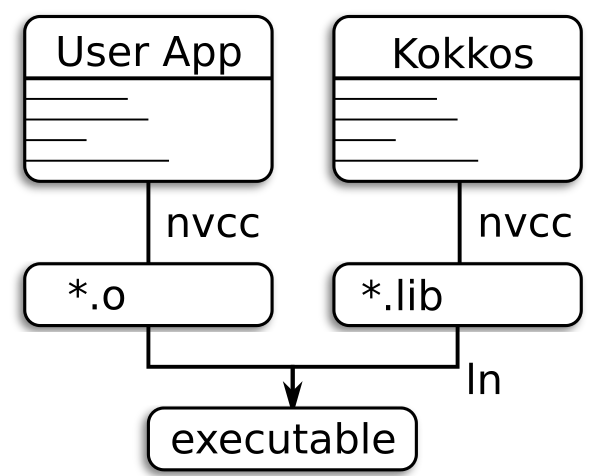
\includegraphics[width=0.3\textwidth]{img/Build.png}}
\caption{Building workflow}
\label{fig}
\end{figure}